\section{Question 3}
Calculate the value of \(\frac{\delta^*}{\delta_{FS}}, \frac{\theta}{\delta_{FS}}$,H,$\sqrt{Re_x}\frac{C_f}{2}$, fro the given
values of m using analytical Thwaits method and compare with the numerical solution of Falkner Skan equation.

\vspace{0.5cm}
\textbf{SOLUTION}
\vspace{0.5cm}

\par The procedure followed for computing given variables using Thwait's method is
given below.\\

\par The given velocity profile is assumed to be governed by power-law, i.e., $u_e(x) = A x^m$ \\

\par Then the following equation is used to compute the momentum thickness
from the velocity profile.
\begin{align*}
    \frac{\theta^2}{\nu} &= \frac{0.45}{u_e^6}\int{}{}u_e^5 dx \\
    \frac{\theta^2}{\nu} &= \frac{0.45 x^{1-m}}{A \left(5m+1\right)}
\end{align*}

\par The nondimensional distance parameter $\lambda$ is then calculated as follows.

\begin{align*}
    \lambda &= \frac{\theta^2}{\nu} \frac{d u_e}{dx} \\
            &= \frac{0.45 m}{5 m + 1}
\end{align*}

\par Then, the values of $H$ and $T$ are computed using the given approximate
expression as
\begin{align*}
    H(\lambda) &= 2.62 - 4.1 \lambda + 14 \lambda^3 + \frac{0.56\lambda^2}{(\lambda+0.18)^2} \\
    T(\lambda) &= 0.22 + 1.52 \lambda - 5 \lambda^3 - \frac{0.072 \lambda^2}{(\lambda + 0.18)^2}
\end{align*}

\par Using, the values of $H$ and $T$ computed above, the following values
were computed.
\begin{align*}
    H &= \frac{\delta^*}{\theta} \rightarrow \delta^* = H \theta \\
    \frac{\delta*}{\delta_{FS}} &= H \sqrt{\frac{0.45}{5m+1}} \\
    \frac{\theta}{\delta_{FS}} &= \sqrt{\frac{0.45}{5m+1}}
\end{align*}

\par Lastly, the nondimensional shear stress is computed as follows.
\begin{align*}
    \tau &= Re_\theta \frac{C_f}{2} \rightarrow \sqrt{Re_x}\frac{C_f}{2} = \frac{T}{\left(\frac{\theta}{\delta_{FS}}\right)}
\end{align*}

\par The computed analytical values were compared with the above computed
numerical values in \Cref{plot_a_1,plot_a_2,plot_a_3,plot_a_4,plot_a_5}. \\

\begin{figure}
   \centering
    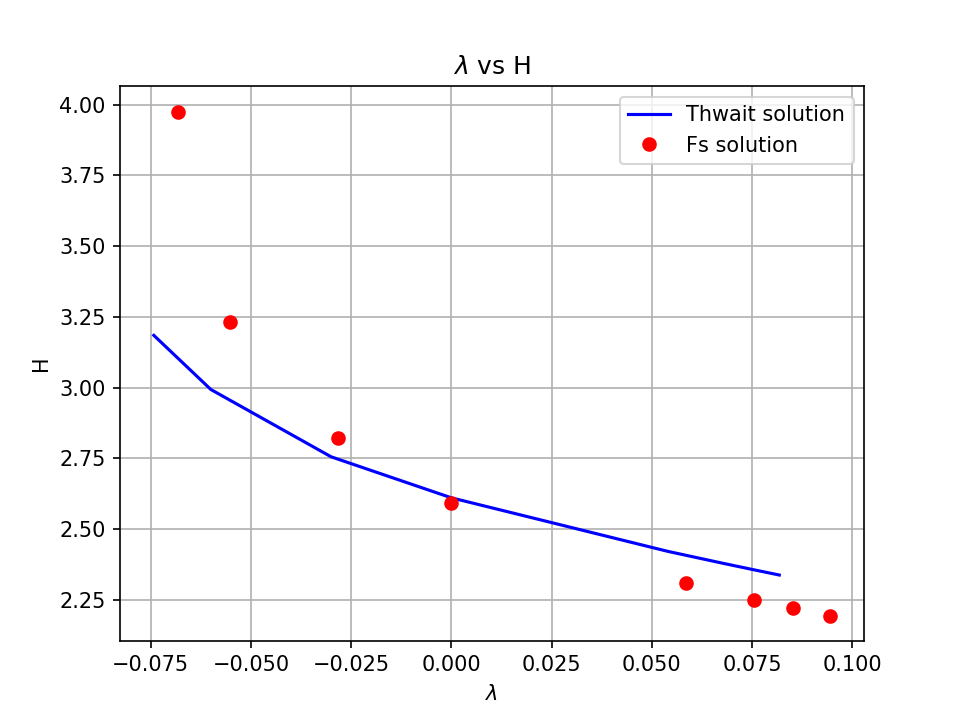
\includegraphics[scale=0.5]{supporting_documents/02_question_2_and_3_codeDevelopment/03_postProcessing/lambda_vs_H_thwait.png}
    \caption{ $\lambda$ vs $H$}
    \label{plot_a_1}
\end{figure}

\begin{figure}
   \centering
    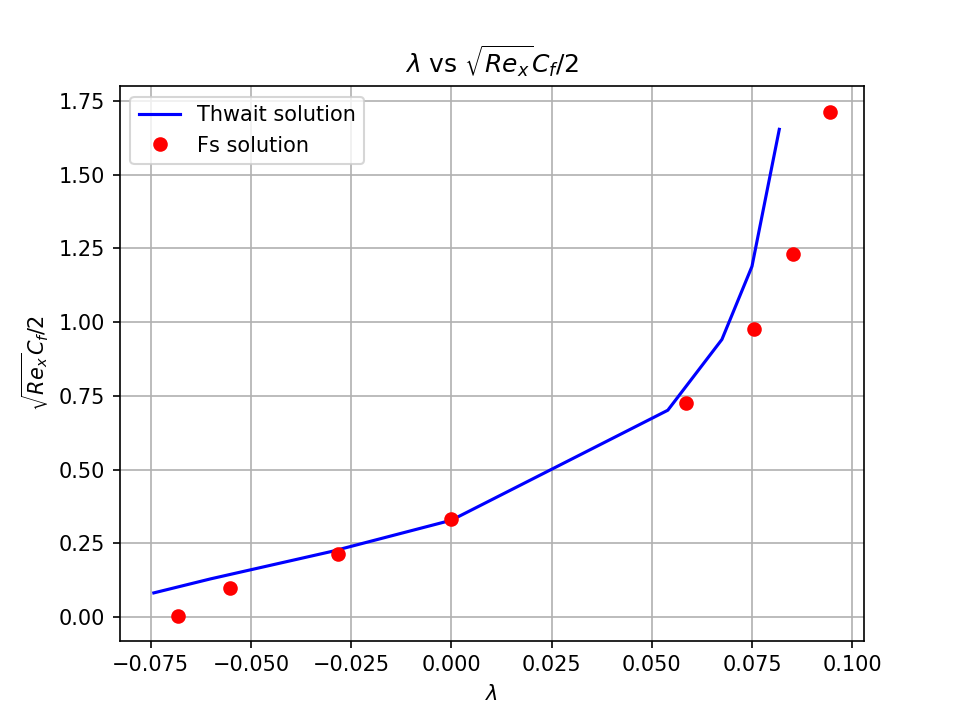
\includegraphics[scale=0.5]{supporting_documents/02_question_2_and_3_codeDevelopment/03_postProcessing/lambda_vs_Rex_Cf_thwait.png}
    \caption{ $\lambda$ vs $\sqrt{Re_x}\frac{C_f}{2}$}
    \label{plot_a_2}
\end{figure}

\begin{figure}
   \centering
    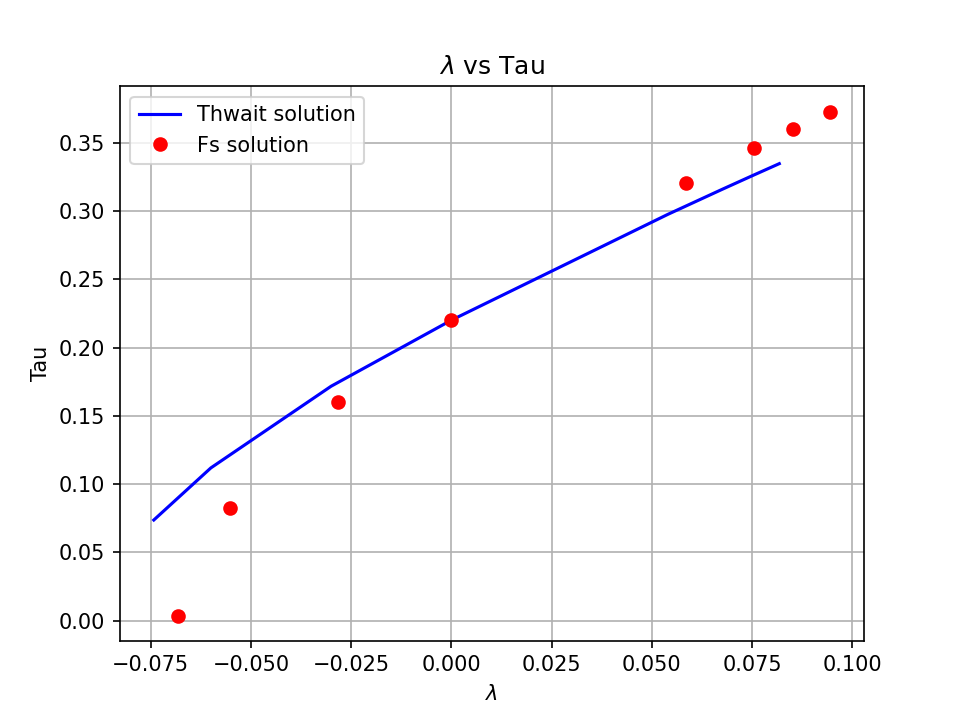
\includegraphics[scale=0.5]{supporting_documents/02_question_2_and_3_codeDevelopment/03_postProcessing/lambda_vs_Tau_thwait.png}
    \caption{ $\lambda$ vs $T$}
    \label{plot_a_3}
\end{figure}

\begin{figure}
   \centering
    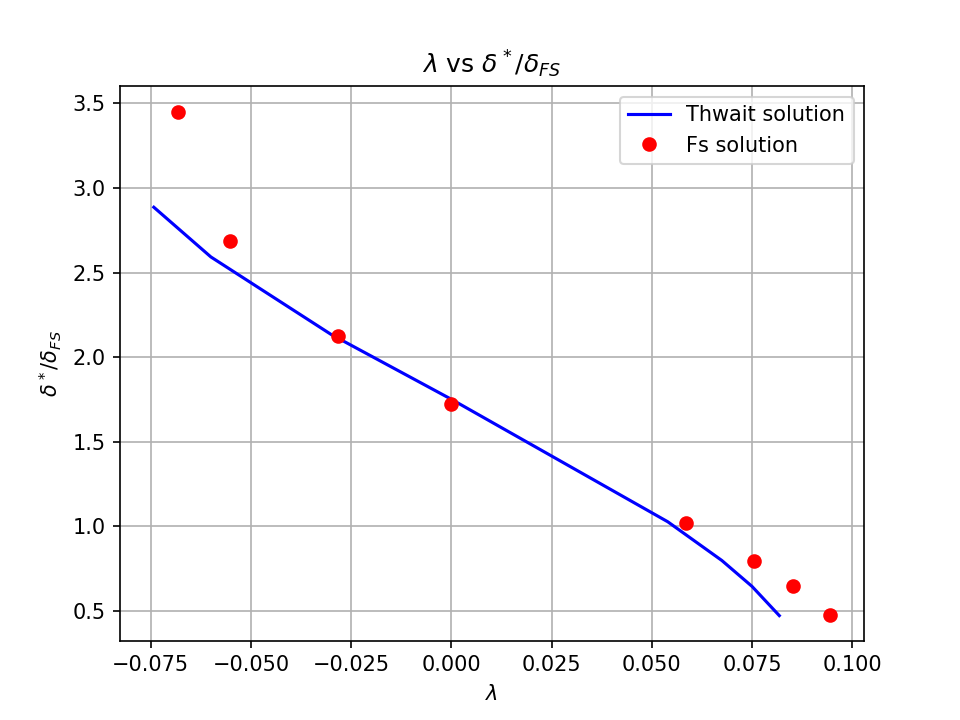
\includegraphics[scale=0.5]{supporting_documents/02_question_2_and_3_codeDevelopment/03_postProcessing/lambda_vs_d_star_dFS_thwait.png}
    \caption{ $\lambda$ vs $\frac{\delta^*}{\delta_{FS}}$ }
    \label{plot_a_4}
\end{figure}

\begin{figure}
   \centering
    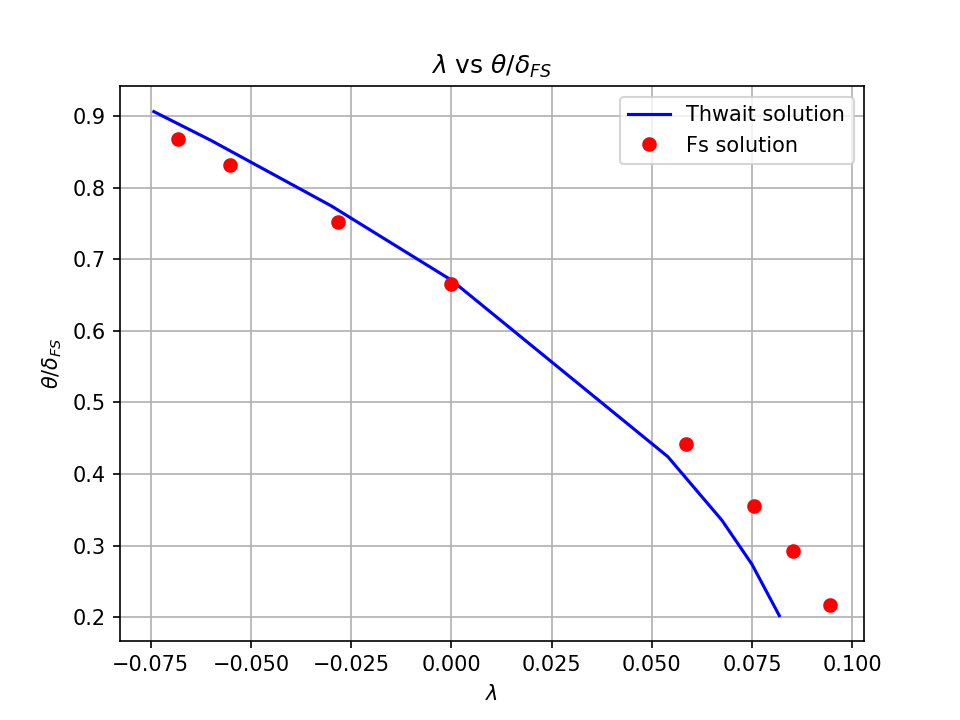
\includegraphics[scale=0.5]{supporting_documents/02_question_2_and_3_codeDevelopment/03_postProcessing/lambda_vs_theta_dFS_thwait.png}
    \caption{ $\lambda$ vs $\frac{\theta}{\delta_{FS}}$}
    \label{plot_a_5}
\end{figure}

\par It can be seen that the Thwait solution does not match well with the
numerical solution, but it is sufficient enough for the preliminary
computations. The \emph{Python} code developed for this post-processing
is given in \Cref{pp_code}.

\pagebreak
